\begin{table*}[th]
\caption{Five Original Datasets}
\centering
\begin{tabular}{|c|l|r|r|r|r|} \hline
Dataset	& Description & Records & Dom. Size & Sens. items & Non-Sens. items  \\ \hline \hline
BMS-POS(POS) &Point-of-sale data from a large electronics retailer    &515597 & 1657&1183355 &  2183665\\ \hline
BMS-WebView(WV) &Click-stream data from e-commerce web site  &77512 & 3340& 137605 & 220673  \\ \hline
Retail &  Retail market basket data   & 88162&16470 &340462 & 568114  \\ \hline
Syn-1 & Synthetic data with cutoff = 121   & 100000& 10000& 408129&  612196 \\ \hline
Syn-2 & Synthetic data with cutoff = 50   & 493193 &5000 &828435 & 1242917 \\ \hline
\end{tabular}
\label{tab:datasets}
\end{table*}

\begin{figure*}[th]
\flushleft
\subfigure[POS]{
\begin{minipage}[c]{0.19\textwidth}
\flushleft
  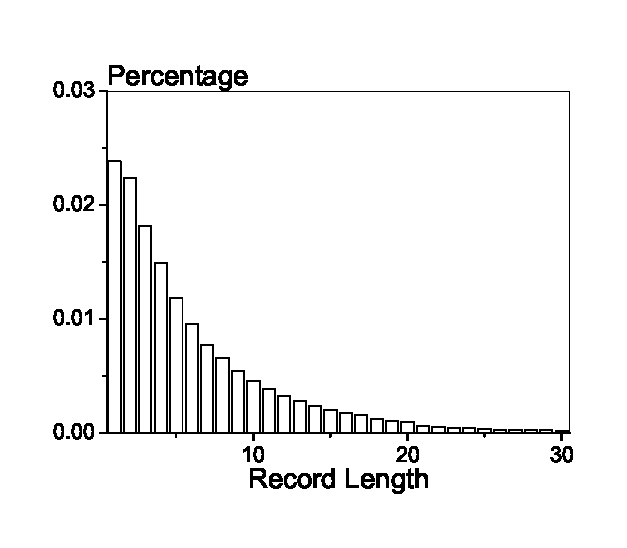
\includegraphics[width=3.8cm]{BMS-POS.eps}
\end{minipage}%
}
\subfigure[WV]{
\begin{minipage}[c]{0.19\textwidth}
\flushleft
  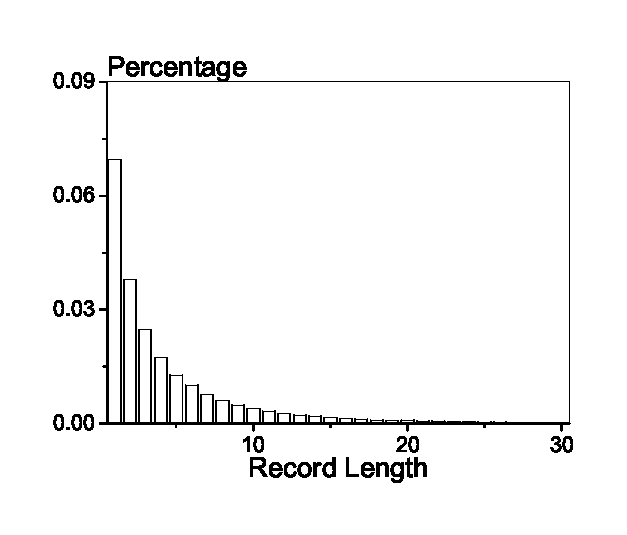
\includegraphics[width=3.8cm]{BMS-WEB.eps}
\end{minipage}%
}
\subfigure[Retail]{
\begin{minipage}[c]{0.19\textwidth}
\flushleft
  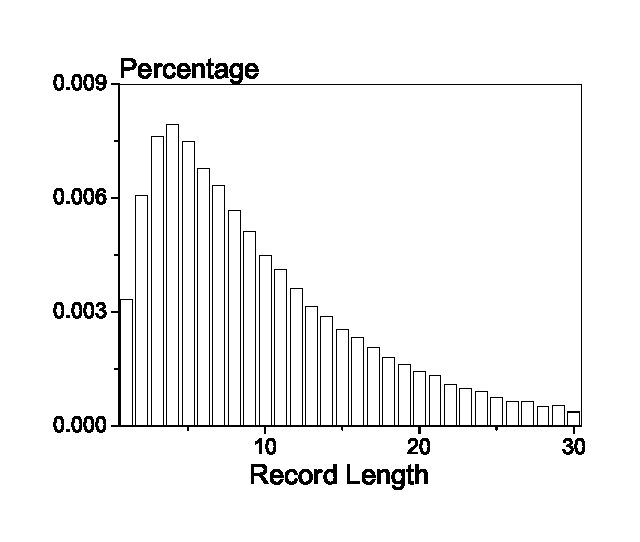
\includegraphics[width=3.8cm]{retail.eps}
\end{minipage}%
}
\subfigure[Syn-1]{
\begin{minipage}[c]{0.19\textwidth}
\flushleft
  \includegraphics[width=3.8cm]{r10w.eps}
\end{minipage}%
}
\subfigure[Syn-2]{
\begin{minipage}[c]{0.19\textwidth}
\flushleft
  \includegraphics[width=3.8cm]{r50w.eps}
\end{minipage}%
}
\caption{Distribution in Record Length of Five Original Datasets}\label{fig:datasets}\shrink
\end{figure*}


\begin{figure*}[th]
\flushleft
\subfigure[POS]{
\begin{minipage}[c]{0.19\textwidth}
\flushleft
  \includegraphics[width=3.8cm]{itembms.eps}
\end{minipage}%
}
\subfigure[WV]{
\begin{minipage}[c]{0.19\textwidth}
\flushleft
  \includegraphics[width=3.8cm]{itemwv.eps}
\end{minipage}%
}
\subfigure[Retail]{
\begin{minipage}[c]{0.19\textwidth}
\flushleft
  \includegraphics[width=3.8cm]{itemretail.eps}
\end{minipage}%
}
\subfigure[Syn-1]{
\begin{minipage}[c]{0.19\textwidth}
\flushleft
  \includegraphics[width=3.8cm]{itemr10w.eps}
\end{minipage}%
}
\subfigure[Syn-2]{
\begin{minipage}[c]{0.19\textwidth}
\flushleft
  \includegraphics[width=3.8cm]{itemr50w.eps}
\end{minipage}%
}
\caption{Distribution in Item Frequency of Five Original Datasets}
\shrink
\label{fig:datasets2}
\end{figure*}

\section{Experimental Results}
\label{sec:eval}

To evaluate our partial suppression algorithm and understand the effects of
various parameters in the algorithm, we conducted a series of experiments
on 5 main datasets in Table \ref{tab:datasets}. BMS-POS and
BMS-WebView are introduced in \cite{Zheng:2001:RWP:502512.502572} and are
commonly used for data mining. Retail is the retail market basket data
provided by an anonymous supermarket store \cite{brijs99:retailData}.
Syn-1 and Syn-2 are synthetic data in which each item is generated with
equal probability, and max record lengths are 121 and 50, respectively.
Figure \ref{fig:datasets} and \ref{fig:datasets2} show
the record length distribution and the item frequency distribution of the five
 datasets. We randomly designate 40\% of the item types in each dataset as
sensitive items and the rest of the items are non-sensitive.
%We also create another five datasets by setting cutoff to fifty.
%\KZ{Explain how we obtain these datasets. Cite the relevant sources.
%Say how we synthesize the Syn-1 and Syn-2. And say something about cutoff=5
%version of the dataset.}
%\XH{Chao Explained below}

We compare our algorithms with the state-of-the-art global suppression
algorithm (named Global) and generalization algorithm (named TDControl) of
Cao {\em et al.}
\cite{Cao:2010:rho}.\footnote{The source code of these algorithms
was directly obtained from Cao.}
In the rest of the section, by ``global suppression'' and
``generalization'', we mean these two algorithms.

Some of the original datasets takes too long to run on
TDControl or global suppression. To enable the comparison in rule
mining, we preprocessed the original datasets into
five additional datasets which contain only records of no more than
five items, and annotate such datasets with ``cutoff = 5''.

In all experiments, we impose a time limit of
2 hours, and experiments that failed to complete by 2 hours is marked
as ``N/A'' or a zero-height bar in the bar charts.
 %However, both TDControl and global
 %suppression are unavailable in large datasets, thus we cannot make %comparisons in Syn-1 and Syn-2 and Retail where $\rho=0.3$
 %with them.


%reported by Cao \etal \cite{Cao:2010:rho}
%against the same data sets.
%Cao {\em et al.} were very supportive of our work and gave us their code directly.
Our experiments were done on an Intel 16-core 2.4GHz machine with
8 GB RAM running Linux kernel 2.6.34. All algorithms are
implemented in C++ on GCC version 4.5.0.
All experiments effectively use just one core since programs are single
threaded, except for the experiment in Section \ref{sec:eval:performance}
where we demonstrate the result of a multi-threaded version of
\PartialR in Table \ref{tab:timeresult}.

%We have 3 real data sets and 2 synthetic data sets in total.
%Prepare the data in large, medium and small sizes. Compare our algos
%with the competing algorithms in rho-uncertainty paper against all
%data sets. Record the time, number of items suppressed, relative entropy,
%and number of rules learned in each of the experiments.
%
%Scaling test: divide the 3 real data sets into 10 parts, and run
%our algos on 10\%, 20\%, 30\%, ... of the whole data sets and plot
%diagram of time and quality of solution.
%
%Add more??

%\begin{itemize}
%\item Explain the implementation of the three variants of our partial algorithm
%(i.e., Partial(R), Partial(L) and Partial(ALL)).
%Explain any implementation details that were not covered by
%the algorithm section. Say how we pick the different params for the algorithm
%and any heuristics options, e.g., random, long record first, long qids first,
%etc.
%\item Explain the implementation details of two of our competitors, TDControl
%and global suppression. How we obtained the code.
%Anything special about the implementation that is different from
%the $\rho$-uncertainty paper.
%
%\item Compare the results in information loss (explain the different metric
%in information loss between us and TDControl), symmetric relative entropy
%(explain what it is and cite) and number of association rules mined. Explain
%the cutoff time of 2 hours in our experiments. That is if the experiment
%exceeds 2 hours, we kill the program. Discuss how we outperform the other
%competitors and why.
%
%\item Compare our results with the optimal solution on small datasets. Explain
%how we get the small dataset first. I think we wanna say it's a subset of
%the cutoff=5 version. Is that true? Discuss why our results are not far
%from the optimal.
%
%\item Discuss the how the iterative algorithm fixes the unsafe qids and how
%bad is the regression. How many iterations are there for a typical dataset?
%How long does each iteration take?
%
%\item Show the scalability results of our algorithms on 3 datasets.
%
%\item Discuss the effects of varying the buffer size $b$ on execution time
%and information losses.
%
%\item Discuss the effects of varying estimated cost bound on the number
%of partitions created, execution time, and info loss.
%
%\item Discuss the effects of varying long record bound on execution time
%and information losses.
%
%\item Discuss the effects of varying long record processing (1000 each time)
%on execution time and information losses.
%\KZ{Do we still have these results?}
%
%\item Discuss the effects of preprocessing (cutting long records).
%\KZ{Do we still have these results?}
%
%\item Give a little summary to this section.
%\end{itemize}
%
%\KZ{END OF OUTLINE.}

%We used 5 datasets in our experiment. BMS-POS and
%BMS-WebView are introduced in \cite{Zheng:2001:RWP:502512.502572} and are
%commonly used for data mining. Retail is the retail market basket data
%provided by an anonymous supermarket store \cite{brijs99:retailData}.
%Syn-1 and Syn-2 are artificially synthetic data by us according to the
%standard that items are made even distributed.
%Figure \ref{fig:datasets} shows the general distribution of the five
% datasets. We see that long records account for only a small portion among
%  all datasets.
%  and the distribution of Retail has a outstanding ascending curve
%  from record length one to record length four, then goes down as others do
%  in longer record length. While Retail dataset also contains more
%  percentage of records with the same small length compared with
%   other four datasets.
  %Although some anomalies exists in retail, it remains the distribution when the record length comes to four.
%  It's reasonable to be explained that
%  customers usually buy more than one goods when they go shopping.
%  To make some comparison possible, like comparing the rules mined
%  from results of all algorithms, we cut off original datasets into
%  other five corresponding datasets which contain only records no more than
%  five items, like Retail(cutoff=5) or Syn-1(cutoff=5). We also create
%  another five datasets by setting cutoff to fifty.

We did some preliminary experiments on the 8 heuristics mentioned in Section
\ref{sec:sanitize}, but found that no single heuristics has
particular advantages over others, and thus choose to fetch
the\qid and pick the record to suppress {\em randomly}.

In what follows, we first present result in data utility, and then
the performance of the algorithms, before finally evaluating the
effects of changing various parameters in partial suppression algorithms.
Unless otherwise noted, we use the following default parameters:
$b_{max} = 10^6$ , $t_{max}$ = 400 secs,
 $\lmin=12$, $\dnum = 1000$. Divide-and-conquer parameters
 $\alpha$, $\beta$, $\gamma$ in Equation (\ref{eq:costfunc}) are learned to
be 1.71E-8, 1.49E-5 and 3.06, respectively.

%Apart from these above parameters, we compare the performance of
%three partial suppression policies (\PartialR, \PartialL and \PartialALL).

  %in order to prove that deleting only sensitive items is the best choice.
%The function
%of these three heuristics is specifically introduced before and we also tested them separately.
%Although some heuristics work in
%some data sets, the general performance of these three methods are almost the same.
% Given that randomness is the most
% simpleness way to solve this problem, we choose the method of randomly picking eventually to present.
%
 %\subsection{Competitors}
%\KZ{Move this subsection to the beginning of the section where we
%talked about Cao's implementation.}

 %Here we introduce the latest work of the global suppression and TDControl of  Cao {\em et al.} \cite{Cao:2010:rho}
 % as the competitors, because they represents a standard global suppression and generalization method based on the greedy algorithm.
 %We also set a cutoff time of 2 hours to prevent the program from running for too long. However,both TDControl and global
 %suppression are unavailable in large datasets,thus we cannot make comparisons in Syn-1 and Syn-2 and Retail where $\rho=0.3$
 %with them.

\subsection{Data Utility}\label{sec:eval:datautility}
We first compare the utility of the anonymized data produced by \PartialR,
global suppression and TDControl in terms of information loss, data distribution,
and association rule mining.

\subsubsection{Information Loss}\label{sec:eval:infoloss}

\begin{figure}[th]
\flushleft
\subfigure[ $\rho=0.3$]{\label{fig:loss-a}
\hspace{-4mm}
\begin{minipage}[c]{0.23\textwidth}
\flushleft
  \includegraphics[width=4.7cm]{3avgloss.eps}
\end{minipage}%
}
\subfigure[ $\rho=0.7$]{\label{fig:loss-b}
\begin{minipage}[c]{0.23\textwidth}
\flushleft
  \includegraphics[width=4.7cm]{7avgloss.eps}
\end{minipage}%
}
\caption{Comparative Results in Information Loss}\label{fig:loss}
\end{figure}

The first comparison is based on information loss (Definition
 \ref{def:infoloss}).
To enable comparison with TDControl which generalizes items in addition to
suppressions, we adopt a more general information loss metric \cite{Cao:2010:rho}:
\[ IL(T,T^\prime)=\frac{\sum_{e\in D}sup(e)\cdot Loss(e)}{\sum_{e\in D}sup(e)}\]
where
\[ Loss(e)=\begin{cases}
  \frac{leaves(n)}{Dom(n)}, & \text{if item $e$ is generalized to node $n\in\mathcal{H}$}\\
  1,                          & \text{if item $e$ is suppressed.} \\
\end{cases} \]
Note this definition is the same as Definition \ref{def:infoloss}
if there is only suppression.

From Figure \ref{fig:loss},
we conclude that \PartialR is uniformly better among the three techniques.
It suppresses only about 26\% items in POS and WV and about 35\% items in
Retail, while Global and TDControl
incur on average 10\% more losses than \PartialR, and up to 75\% losses
in the worst case.
Note Global and TDControl failed to complete with some datasets.
This confirms that \PartialR causes less information losses than peers.

%indicating that our algorithm has a
%strong flexibility in $\rho$.

\subsubsection{Data Distribution}\label{sec:eval:datadistribution}

\begin{figure}[th]
\flushleft
\subfigure[ $\rho=0.3$]{
\hspace{-4mm}
\begin{minipage}[c]{0.23\textwidth}
\flushleft
  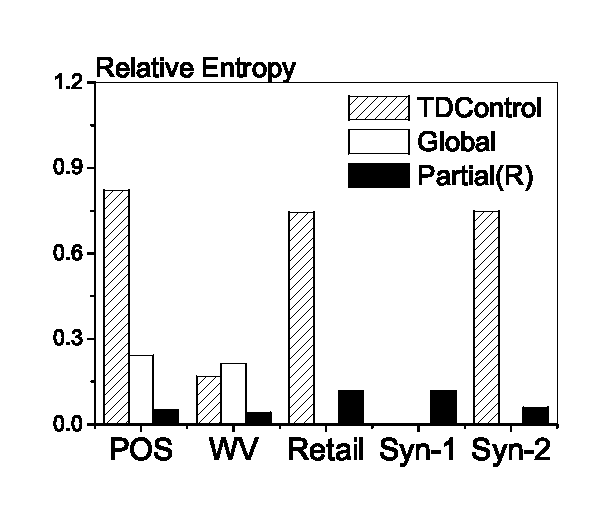
\includegraphics[width=4.5cm]{3relative.eps}
\end{minipage}%
}
\subfigure[ $\rho=0.7$]{
\begin{minipage}[c]{0.23\textwidth}
\flushleft
  \includegraphics[width=4.5cm]{7relative.eps}
\end{minipage}%
}
\caption{Comparative Results in Symmetric Relative Entropy}
\label{fig:entropy}
\end{figure}

To determine the similarity between the item frequency distribution
of original data and that of the anonymized data,
we use the symmetric relative entropy between the two distributions.
The ordinary relative entropy
\cite{Lin91divergencemeasures} which is also called Kullback-Leibler
divergence is defined as follows.
\begin{equation} \label{eq:relative}
\mathcal{R}(H_1||H_2)=\sum_{i=1}^{n}H_1(i)\cdot log(H_1(i)/H_2(i))
\end{equation}
where $H_1$ and $H_2$ are two histograms and each $H_1(i)$ and $H_2(i)$ represent the height of the corresponding bar in $H_1$ and $H_2$ respectively.
To prevent zero denominators, we modified (\ref{eq:relative})
to a symmetric relative entropy \cite{Fisher:2008:DSF} defined as
\[\mathcal{S}(H_1||H_2)=\frac{1}{2}\mathcal R( H_1||H_1 \oplus H_2)+\frac{1}{2}\mathcal R( H_2||H_1 \oplus H_2)\]
where  $H_1 \oplus H_2$ represents the union of the $H_1$ and $H_2$.

Figure \ref{fig:entropy} shows that \PartialR outperforms the peers
as the distribution of its output has the highest resemblance
to the original datasets.
On the contrary, TDControl is the worst performer
since generalization algorithm creates a lot of new items while
suppressing too many item types globally.
%Results of global suppression are five times more than
%those of \PartialR on average,
%despite its relatively higher similarity
%than results of TDControl.

%  The anomaly in WV when {$\rho$} is 0.3 dues to the uncertainty of global suppression method. Figure \ref{fig:entropy}
%illustrates that relative entropy of partial(R) is five times less than both TDControl and global suppression, indicating that the
%remaining distribution is much more similar with the original distribution
%than TDControl and global suppression is.

\subsubsection{Association Rules Mining}\label{sec:eval:rulemining}
The most common criticism of partial suppression is that it
changes the support of good rules in the data and introduces spurious
rules in rule mining. In this experiment, we test the algorithms on
data sets with cutoff = 5, and check the rules mined from the anonymized data
with support of 5. Mining rules from the original datasets with many
long records is prohibitive due to large memory requirements.

Table \ref{tab:rules} gives the results. The ``Original'' row records the
number of rules that can be mined from the original data. ``Spurious \%''
denotes the percentage of the inferred rules that are extraneous.
Both TDControl and Global performs badly in this category, with
negligible number of original rules remaining after anonymization.
Conversely, all of of the partial
suppression algorithms manage to retain most of the rules, with only a
fraction (about 20\%) of which are spurious. We argue that for downstream
rule mining applications, results from Global are almost
useless even though it introduces no extra rules. On the other hand, TDControl
is only useful if the generalization hierarchy is recognized by the data user.
Note that these new, more general rules from the result of TDControl can be
``specialized'' into rules of original level in the generalization hierarchy.
For example, we can specialize a rule \{dairy product $\rightarrow$ grains\}
into
\{milk $\rightarrow$ wheat\},
\{milk $\rightarrow$ rice\},
\{yogurt $\rightarrow$ wheat\},
\{yogurt $\rightarrow$ rice\}, etc.
%However, the newly generated rules only account for a small part
%in the rules mined from result of
%\PartialR and what matters more is that remained rules still occupy a
%large portion compared with the original rules based on the experiment
%result in Table \ref{tab:rules}. New rules may also be generated by
%generalization, since the domain of the generalized dataset
%is different from the original one. A reasonable way
%to transfer the newly generated rules by generalization is to
%replace the newly generalized item with specific items which are its
%descendants. For example, if there exists a generalized rule
%$\{1\ 2\ 3\rightarrow \alpha\}$ where $1=\{b\ c\}, 2=\{d\},
%3=\{e\ f\}$, we can transfer this rule into four different rules such
%as $\{b\ d\ e\rightarrow \alpha\}$,  $\{b\ d\ f\rightarrow \alpha\}$,
%$\{c\ d\ e\rightarrow \alpha\}$, $\{c\ d\ f\rightarrow \alpha\}$.
%Through this strategy, we can now compare rules mined from the result
%of TDControl and \PartialR in the same level of item domain.
Take BMS-POS(cutoff = 5) for an example. 36 generalized rules are
mined from TDControl result. After specializing we get
438053 possible rules with only 2 of them in the original rules!
% So there are 438051 spurious rules!
% This reflects that the support of rules become higher
% after items being generalized, which leads to the fact that
% the newly generated rules is confirmed to exist in original rules only
% when support is set to 1, but meaningless when support is higher.Another
% thing is if data users don't agree on the generalized hierarchy,
% generalized rules are also meaningless.

%table for rules (sup=5 rho=0.7)
\begin{table}[th]
\caption{Association Rules Mined with Support $5$ ($\rho=0.7$)}
\centering
\begin{tabular}{|l|r|r|r|}
  \hline
  % after \\: \hline or \cline{col1-col2} \cline{col3-col4} ...
   & POS & WV  & Retail \\
 & (cutoff = 5) &(cutoff = 5) & (cutoff = 5) \\\hline \hline
 Original & 4457 & 600 & 674 \\\hline
  TDControl& 36 & 58 & N/A \\
 (Spurious \%) & (100\%) & (100\%) & N/A \\\hline
Global & 5 & 98 & 87\\
(Spurious \%) & (0\%) & (0\%) & (0\%)\\\hline
  \PartialR & {\bf 4007} & {\bf 249} & {\bf 402} \\
(Spurious \%) & {\bf (22\%)} & {\bf (16\%)} & {\bf (23\%)}\\\hline
 \PartialL & 3087 &199 & 251\\
(Spurious \%) & (28\%) & (25\%) & (17\%)\\\hline
 \PartialALL & 3335 &243 & 335\\
(Spurious \%) & (27\%) & (22\%) & (20\%)\\\hline
\end{tabular}
\label{tab:rules}
\end{table}

\subsubsection{Comparison with Optimal Solutions}\label{sec:eval:optimal}

\begin{table}[th]
\caption{Optimal Datasets}
\centering
\begin{tabular}{|l|r|r|}
  \hline
  % after \\: \hline or \cline{col1-col2} \cline{col3-col4} ...
     & Opt-1 & Opt-2 \\  \hline \hline
  Records & 15 & 25 \\  \hline
  Domain Size & 10 & 16 \\  \hline
  Sensitive items & 28 & 28 \\  \hline
   Non-Sens. items & 47 & 86 \\
  \hline
\end{tabular}
\label{tab:optimaldatasets}
\end{table}

In this part, we want to evaluate how far is our anonymized solution from the
{\em optimal solution}, defined in Definition \ref{def:osp}.
Because we obtain the optimal solution by brute force enumeration of all
possible suppressions, the search space is extremely large.
We therefore created two tiny synthetic datasets, Opt-1 and Opt-2,
for the sole purpose of this experiment, and their characteristics are listed in
Table \ref{tab:optimaldatasets}.
Table \ref{tab:optimal} compares the results of three algorithms against the
optimal solution on the two datasets. All three algorithms finishes in a few
millisecond, but in terms of information loss, \PartialR is a clear winner. In fact
for Opt-2, it achieves the optimal solution! This experiment also illustrates
the hardness of the optimal suppression problem.

%We also put the result incurred by global suppression and
% TDControl as a reference. The optimal result is calculated through exhaust algorithm and
% the time cost is almost unacceptable.
%  While our result got a very close result in short time.
%  Such huge differences between partial suppression algorithm
% and the other two algorithms suggest the superiority of our algorithm.

\begin{table}[th]
\caption{Comparison with Optimal Result ($\rho=0.7$)}
\centering
\begin{tabular}{|l|r|c|r|c|c|} \hline
\multirow{2}{*}{Algorithm}& \multicolumn{2}{c|}{Opt-1}& \multicolumn{2}{c|}{Opt-2}\\\cline{2-5}

& Info Loss &Time & Info Loss&Time \\ \hline\hline
Optimal &0.20 &  67 hours &0.18 &214 hours\\ \hline
TDControl  &0.37  &$<$10ms& 0.36 &$<$10ms\\ \hline
Global  & 0.41 &$<$10ms& 0.33&$<$10ms \\ \hline
\PartialR  &{\bf 0.23} & {\bf $<$10ms} & {\bf 0.18} & {\bf $<$10ms} \\ \hline
\end{tabular}
\label{tab:optimal}
\end{table}


\subsection{Performance}\label{sec:eval:performance}
In this section, we evaluate the time performance and scalability of
the algorithms and analyze the regression in \PartialR.

\subsubsection{Time Performance}\label{sec:eval:time}
\begin{table}[th]
\caption{Comparison in Time Performance ($\rho=0.7$)}
\centering
\begin{tabular}{|l|r|r|r|r|r|}
  \hline
  % after \\: \hline or \cline{col1-col2} \cline{col3-col4} ...
  Algorithm & POS & WV & Retail & Syn-1 &Syn-2 \\  \hline \hline
  TDControl & 183 & 30 & 156 & N/A&   476  \\  \hline
  Global & 1027 & 81 & 646 & N/A &  N/A  \\  \hline
%  \PartialR & 6582 & 305 & 1497 & 323&761 \\\hline
  \PartialR$^{5}$ & 1355 & 146 & 272 &  179 & 461\\ \hline
  \PartialR$^T$ & {\bf 50} & {\bf 15}& {\bf 19} & {\bf 12}& {\bf 36} \\ \hline
  \end{tabular}
\label{tab:timeresult}
\end{table}

Since data anonymization often take place in offline mode,
time performance is often not critical.
Nonetheless, time matters if we want our algorithm to
scale to large datasets.
%But reasonable time performance is still important for a data user.
From Table \ref{tab:timeresult}, TDControl is the clear winner
for three of the five dataset.
Results for Global are not available for Syn-1 and Syn-2.
Rules mined from the two synthetic data are enormous when support
is 1, as a result, the program run out of memory.
%\PartialR is slower because the default value
%of $t_{max}$ is 400 seconds.
In this experiment, we set $t_{max} = 5$ for \PartialR$^{5}$ and it achieves
very reasonable time performance with significant speed-up gained from the DnC
optimization.

One great advantage of our algorithm is that our DnC optimization
is naturally amenable to coarse-grained data parallelism.
The multi-threaded version (\PartialR$^T$ in Table \ref{tab:timeresult}) showed
significant reduction in execution time for large datasets on
the 16-core machine using the setting $t_{max} = 5$.

% don't use multi-threaded method to implement our algorithm. But our time
% performance is also feasible on POS and Retail data since we set $t_{max}$
% to 400 seconds, and POS is divided into 32 partitions, it costs about 214
% seconds to handle each partition. The same goes for Retail. This also
% reflects that if we set $t_{max}$ to smaller values, our time performance
% will turn better.
%artificially split dataset to the same number of partitions created
% by the real program,
%and simultaneously start same number of partial suppressors on our
%16-core machine to anonymize each partition. We use the
%the maximal time consumed among anonymizing all
%partitions to estimate the time cost if we implement our algorithm
%in multi-threaded manner.
%From the result shown in Tabel \ref{tab:timeresult},
%we can the real efficiency our algorithm can acquire.

% algorithm can be designed as multi-thread program
%, suggesting that the time performance will be divided by a constant according to the number of cores while theirs are only
%single-thread program.

\subsubsection{Scalability}\label{sec:eval:scale}
This experiment illustrates the scalability of our algorithm
w.r.t. data size. Figure \ref{fig:scale:a} shows the result with
DnC, while Figure \ref{fig:scale:b} shows the result
without DnC. Both variants exhibit almost perfectly
linear scale-up on Syn-1 and WV which are not partitioned at all.
On Retail with DnC, data is partitioned into
two pieces at 2/5 data, four pieces at 3/5 and 4/5 data, and then
eight pieces for the whole data. Increasing partitioning causes the algorithm
to witness superlinear speedup in Figure \ref{fig:scale:a}.
%The execution for 3/5, 4/5 and whole of Retail shows almost linear scale-up.
On Retail without DnC, because there are more long records,
the \PartialR shows a {\em slow} sublinear time cost, which is
line with the conclusion of quadratic time complexity 
in Section \ref{sec:analysis}.

%According to Figure \ref{fig:scale:b}, our
%algorithm shows a perfect linear property with regard to the data size,
%suggesting that the time performance of our algorithm
%increases linearly with data size. Two anomalies appear in Figure \ref{fig:scale:a}, which makes sense because we set $t_{max}$ to 400s. As a result, both WV and Syn-1 is not divided but retail is  divided into 2 pieces at 2/5 and 4 pieces at 3/5. Therefore, the
%curve of retail in Figure \ref{fig:scale:a} does not show a perfect linear property but substantiate the significant role played by
%our cost function.

\begin{figure}[th]
\flushleft
\subfigure[With DnC]{\label{fig:scale:a}
\hspace{-4mm}
\begin{minipage}[c]{0.23
\textwidth}
\flushleft
  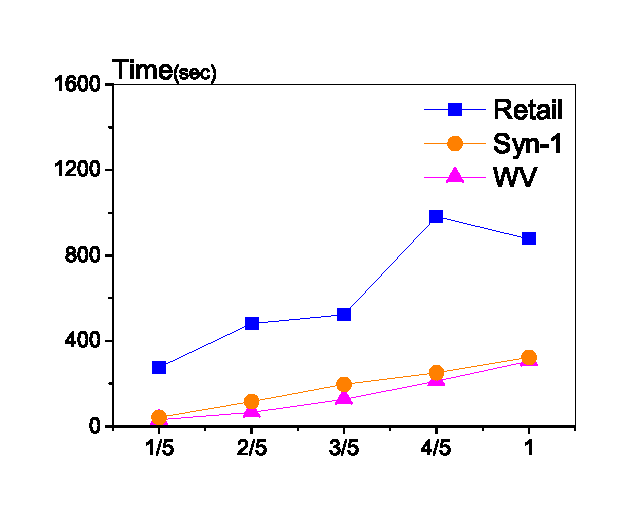
\includegraphics[width=4.7cm]{scaletime.eps}
\end{minipage}%
}
\subfigure[Without DnC]{\label{fig:scale:b}
\begin{minipage}[c]{0.23\textwidth}
\flushleft
  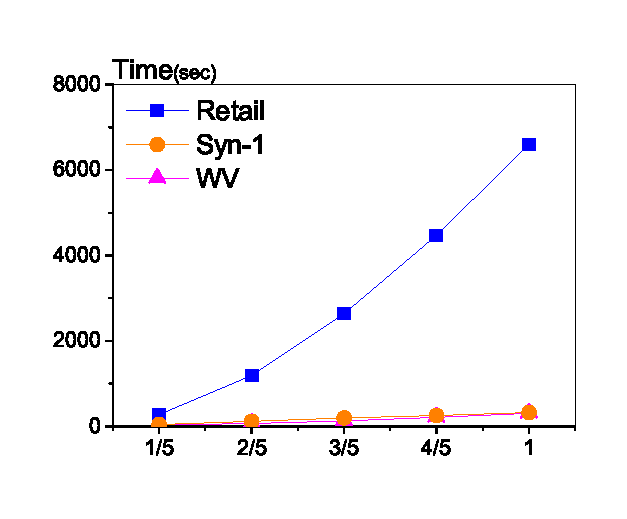
\includegraphics[width=4.7cm]{scaletimeno.eps}
\end{minipage}%
}
\caption{Scale-up with Input Data ($\rho=0.7$)}\label{fig:scale}
\end{figure}

\subsubsection{Regression}\label{sec:eval:regression}
In this part, we trace the regression behavior of \PartialR.
We can estimate the amount of regression by comparing the number of
\qids ever fixed with the number of distinct\qids fixed. The first number
contains repeated \qid fixes. Because the number of\qids in a dataset can be
extremely large especially with very long records. As such we restrict this
experiment to datasets with cutoff = 5.

Table \ref{tab:regression} shows that in all
datasets, differences between the last two columns are very small,
indicating that in practice, very little regression (on average about 0.13\%)
occurred.

Another interesting finding is that the number of distinct\qids fixed
is much smaller than the number of unsafe\qids in the original data (column 2).
On average, fixing one\qid actually causes 4.28 unsafe\qids to be sanitized.
This validates our hypothesis that by suppressing some items to fix one\qid,
the algorithm actually fixes other unsafe\qids at the same time as well.

%?g
%?gWe record the number of original distinct unsafe qids,
%?gthe number of the distinct unsafe qids and the total fixed qids.
%?gShown in Table \ref{tab:regression}, we
%?g find that the  distinct unsafe qids really fixed is much less than the
%?g original unsafe ones. In a conclusion, once a qid is fixed, it
%?g may effect other correlated qids and diminish the number of
%?g   unsafe qids dramatically.
%?g   The average ratio is about 4.28, indicating that one fixed qid will help to fix
%?g another 4.28 qids.
%?g
%?g  Another important characteristic of our algorithm is that the regression just plays a tiny role in our
%?g algorithm.
%?g We choose one qid in the buffer each time and fix it. The regression will work when such fixed qid will break the
%?g previously fixed ones, thus causing the algorithm to recheck the previously fixed ones. However, according to Table \ref{tab:regression} , such
%?g influence only accounts for a tiny part of the total fixed qids, since
%?g The difference between distinct fixed qids and all fixed qids is very small. The average ratio of rechecking qids is only
%?g   $0.13\%$, suggesting that one fixed qid will cause 0.13 previously fixed ones to be unsafe.
%?g

\begin{table}[th]
\caption{Qid Fixing and Regression (\PartialR, $\rho=0.7$)}
\centering
\begin{tabular}{|l|r|r|r|r|r|} \hline
Dataset 	& Orig Qids & Orig Qids &  Qids Fixed  & Qids Fixed   \\
(cutoff=5)	&(Total)  & (Unsafe) &( Distinct)  &(All)   \\ \hline \hline
POS  & 196968 & 111112 & 36888 & 36924\\ \hline
WV  & 82109	&62341	&15437	&15487\\ \hline
Retail  & 129358	&109687	&21789&	21839\\ \hline
Syn-1 & 187273&	177018&	37707&	37707\\ \hline
Syn-2  & 592440	&574145	&123156	&123156\\ \hline
\end{tabular}
\label{tab:regression}
\end{table}

\subsection{Effects of Parameters on Performance}\label{sec:eval:effect}
In this section, we analyze the trade-offs in three variants of our basic
algorithm, and study the effects of $t_{max}$, $b_{max}$ and $\lmin$ on
quality of solution (in terms of information loss) and time performance.
%parameters for optimization defined in our algorithm help to ameliorate the time performance by the largest extent but remain the quality of the suppressed datasets.
%We have 4 different parameters including partial suppression policies

\subsubsection{Partial Suppression Strategies}\label{sec:eval:partialsuppression}
The following experiments to illustrate the result of
different suppression strategies.
Figure \ref{fig:partial} suggests that \PartialR
outperforms the other two different strategies in information loss
and association rule learning (See Table \ref{tab:rules}) but doesn't do
as well in relative entropy. Time performances of the three approaches
are in the same range. We therefore conclude that \PartialR is an overall
winner and use it to compare with TDControl and Global in
other experiments of this section.

\begin{figure}[th]
\centering
  \flushleft
\subfigure[ $\rho=0.7$]{
\hspace{-4mm}
\begin{minipage}[c]{0.23\textwidth}
\flushleft
  \includegraphics[width=4.7cm]{patialinfo.eps}
\end{minipage}%
}
\subfigure[ $\rho=0.7$]{
\begin{minipage}[c]{0.23\textwidth}
\flushleft
  \includegraphics[width=4.7cm]{partialrela.eps}
\end{minipage}%
}
\subfigure[ $\rho=0.7$]{
\hspace{-4mm}
\begin{minipage}[c]{0.23\textwidth}
\flushleft
  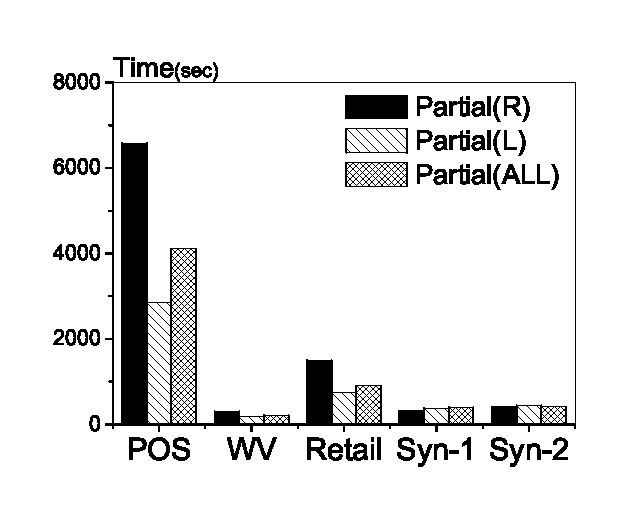
\includegraphics[width=4.7cm]{partialtime.eps}
\end{minipage}%
}
\caption{Comparison among Partial Suppression Strategies}
\label{fig:partial}
%\textit{Partial(R)} suppresses sensitive only, \textit{Partial(L)} suppresses items on left side of a inference, and \textit{Partial(ALL)} suppresses items on both sides of a inference.}\label{fig:fft}
\end{figure}

\subsubsection{Variation of $t_{max}$}\label{sec:eval:timebound}
The value of $t_{max}$ determines the size of a partition in DnC. Smaller
$t_{max}$ can give rise to more partitions. Here, we
evaluate how partitioning helps with time performance and
its possible effects on suppression quality.
Figure \ref{fig:timebound-a} clearly indicates that decreasing the $t_{max}$ and
hence increasing the granularity of DnC doesn't cost us the quality of solution, as
the three lines for Retail, Syn-2 and WV are all flat.

On the other hand,
time cost decreases (note the log scale on both X and Y axes in
Figure \ref{fig:timebound-b}) with decreasing $t_{max}$. For Syn-2 and WV,
partitioning only happens when the $t_{max}$ is small enough. When there is
no change in number of partitions, the curve retains flat.
When there is increasing partitions, as in the case of Retail, the time cost
decreases superlinearly. 
%This can be explained by Equation (\ref{eq:costfunc}).
%As Figure \ref{fig:scale:b} shows,
%the time cost for \PartialR on Retail is a slow exponential function, say
%$\epsilon^{|T|}$ where $\epsilon$ is small. Now, if decreasing $t_{max}$ causes
%a split of data into equal halves. The expected time cost will be
%$2\epsilon^{\frac{|T|}{2}}$. This rough estimation clearly gives rise to
%an exponential speed up.


%Figure \ref{fig:timebound} shows that the time performance increases
%exponentially with the increase of $t_{max}$.However, the quality of our result almost remains the same, which indicates that
%partition is a reasonable method which can be applied to our algorithm.
%The line tends to be plain when $t_{max}$ becomes larger,
%because the expected time is less than $t_{max}$,
% suggesting that no partitions will be executed.

%timebound
\begin{figure}[th]
\flushleft
\subfigure[Information Loss]{
\label{fig:timebound-a}
\hspace{-4mm}
\begin{minipage}[c]{0.23\textwidth}
\flushleft
  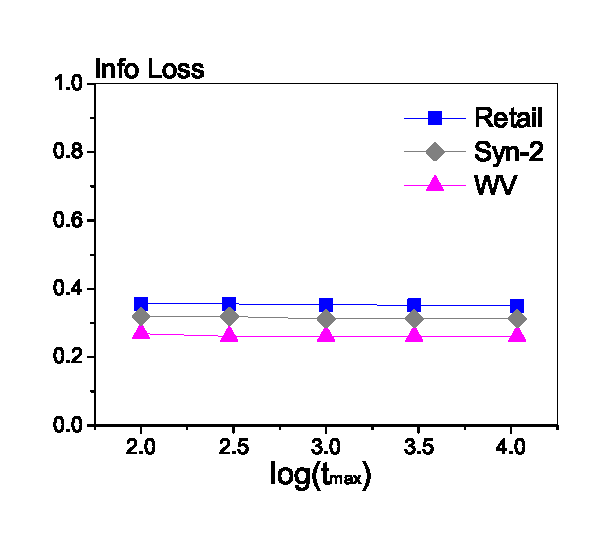
\includegraphics[width=4.7cm]{timebond_avg.eps}
\end{minipage}%
}
\subfigure[Time Performance]{
\label{fig:timebound-b}
\begin{minipage}[c]{0.23\textwidth}
\flushleft
  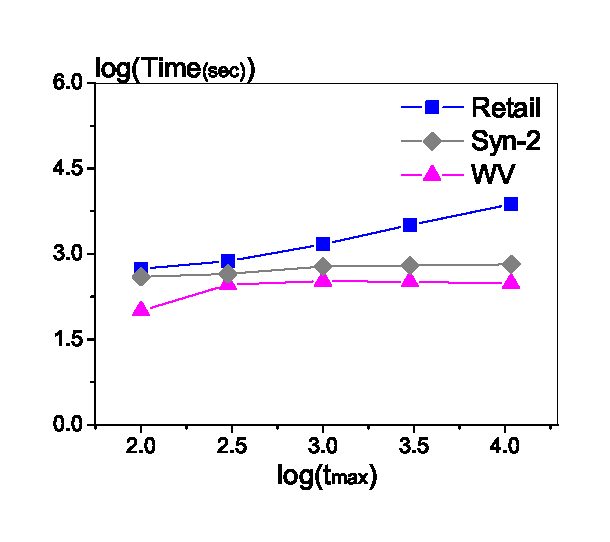
\includegraphics[width=4.7cm]{timebond.eps}
\end{minipage}%
}
\caption{Variation of $t_{max}$ ($\rho = 0.7$)}\label{fig:timebound}
\end{figure}

\begin{figure}[th]
\flushleft
\subfigure[Information Loss]{
\hspace{-4mm}
\begin{minipage}[c]{0.23
\textwidth}
\flushleft
  \includegraphics[width=4.7cm]{buffersizeavg.eps}
\end{minipage}%
}
\subfigure[Time Performance]{
\begin{minipage}[c]{0.23\textwidth}
\flushleft
  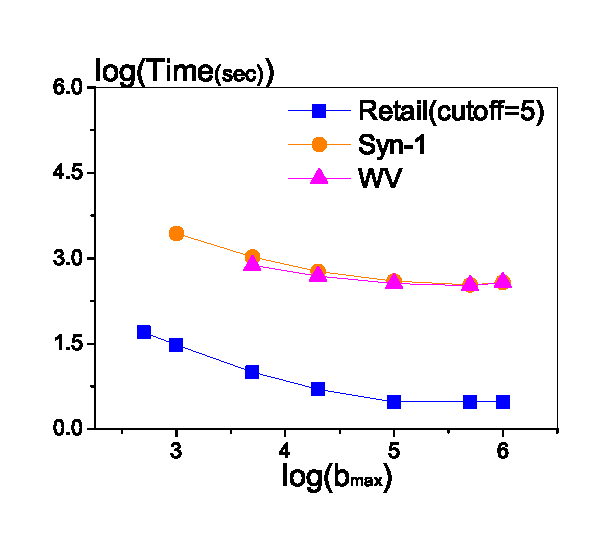
\includegraphics[width=4.7cm]{buffersize.eps}
\end{minipage}%
}
\caption{Variation of Buffer Size $B$ ($\rho=0.7$)}\label{fig:buffersize}
\end{figure}


\subsubsection{Variation of $b_{max}$}\label{sec:eval:buffersize}

This experiment illustrates the impact by $b_{max}$ to performance.
Note first that varying $b_{max}$ has no effect on the information loss which
indicates that this parameter is purely for performance tuning.
At lower values, increasing $b_{max}$ gives almost exponential
savings in running time. But as $b_{max}$ reaches a certain point, the speedup
saturates, which suggests that given the fixed size of the data,
when $B$ is large enough to accommodate all\qids enumerated from
the short records at once, further increase in $b_{max}$ is not useful.
The other purpose of setting a reasonable value for $b_{max}$ is to limit the
amount of memory use.

%exponentially with the decrease of buffer size while the Information loss remains the same.
% The slope also tends to be zero at the end of the curve
%because all of the qids in short records can be put in the buffer at one time,
%thus making the function of buffer less powerful. The function of $b_{max}$ ont only ameliorates the time performance
%.but is
%designed for setting an upper limit of memory capacity

\begin{figure}[th]
\flushleft
\subfigure[Information Loss]{
\label{fig:longrecord-a}
\hspace{-4mm}
\begin{minipage}[c]{0.23
\textwidth}
\flushleft
  \includegraphics[width=4.7cm]{lravgloss.eps}
\end{minipage}%
}
\subfigure[Time Performance]{
\label{fig:longrecord-b}
\begin{minipage}[c]{0.23\textwidth}
\flushleft
  \includegraphics[height=4.1cm,width=4.7cm]{lr.eps}
\end{minipage}%
}
\caption{Variation of $\lmin$ ($\rho=0.7$)}\label{fig:longrecord}
\end{figure}



\subsubsection{Variation of $\lmin$ }\label{sec:eval:longrecord}
%\KZ{We may wanna do more experiments here with smaller $\lmin$. I think we
%will see the dip in the curve for Syn-1 and WV as well given a small enough
%$\lmin$.}
Figure \ref{fig:longrecord-a} first verifies that $\lmin$ is a performance
parameter which doesn't affect the solution quality much.

The value of $\lmin$ essentially determines what portion of the data is handled
as short records and what port is handled as long records.
When $\lmin$ is small, more records are handled by \HandleLongRecord.
Because \HandleLongRecord involves finding intersections between \qid
containers, it can be increasingly expensive with the average size of
long records if there are more frequent itemsets in these records.
This is evident from the result of Retail. Thus we see the
curve goes up to the left.
Divide-and-conquer actually solves this problem to some extent.
If $\lmin$ is not large enough for a certain dataset,
$\sum_{|R| \ge \lmin}\max_{t \in R} \csize(t)$ in Equation (\ref{eq:costfunc})
tends to be very large, which triggers the DnC optimization.

When $\lmin$ is large, more records are handled by \HandleShortRecords.
The complexity of \HandleShortRecords is largely determined by the \Enum function
whose cost increases with the length of the\qids. Therefore, we see to the right
of Retail and also in WV and Syn-1, the curves goes up. One interesting point is
that, for some dataset such as Retail, there exists a particular value
for $\lmin$ which minimizes the time cost, that is, the lowest point in the curves.
%As $\lmin$ increases, more records are handled by \HandleShortRecords.
%In case of Syn-1 and WV which have few records longer than 12, the total cost
%is dominated by \HandleShortRecords which is in turn dominated by \Enum function,
%and increases exponentially with the length of records.
%
%In case of Retail which comes with a lot more records longer than 12, the total
%cost is initially dominated by \HandleLongRecord in which computing the
%intersection of containers is the most expensive part. As we increase $\lmin$
%and move more input records from \HandleLongRecord to \HandleShortRecords,
%the time savings in less intersection computation outweighs the
%additional time costs for enumerating\qids in \HandleShortRecords. As a result,
%as $\lmin$ increases from 12 to 18, the total time cost decreases.
%But as the number of long record diminishes, \HandleShortRecords becomes to
%dominate the suppression process. At a certain point, additional cost in
%enumeration of\qids outweighs the saveings in \HandleLongRecord, and the
%total execution time starts going up.

%The last experiment illustrates the importance of
% $\lmin$ in our algorithm.
%Generally speaking, time performance has exponent relation with $\lmin$,
%since the number of qids increase exponentially
%with the record length.
%On the other hand, Retail has many more longer records, and as such we see
%an interesting turning point in its curve.
%To understand this strange curve, we should
%review the function of $\lmin$ at first. We delete all
%sensitive items in the records where the number of
%non-sensitive items larger than to $\lmin$ to accelerate the program while on the other
%hand we set those records whose length is larger
%than  $\lmin$ as special cases in our
%algorithm.
%When $\lmin$ is small, the cost of intersection operations in \HandleLongRecord
%may exceed the whole scanning cost.
%Therefore, the line in retail drops at first because $\lmin$ is not large
%enough for retail and increases dramatically when  $\lmin$ comes to 20.

%\subsection{Summary}\label{sec:eval:summary}
%Our main purpose is to keep as many items as possible. Just as the
%optimal results in Table \ref{tab:optimal}, finding an optimal solution is
%impossible within limited time. However, results of global suppression
%and generalization algorithm is far from satisfactory.
%Our algorithm outperforms them in information loss, a common metric widely used in previous work, symmetric relative entropy and the remained rules which are defined by us as two important metric of set-valued datasets.
%To optimize our algorithm, we introduce a divide-and-conquer strategy
%and the result shows the effectiveness of this method.
%Although our algorithm is linear with the data size
%, we still try to optimize our algorithm.
%We plot figures by varying those parameters seperately.
% All of those results show a
%common phenomenon that the time performance becomes
% much better but the quality almost remains the same.
%In summary, the experiment result shows that our algorithm
%has a much more promising application prospect than the previous work does.




%\begin{table*}[th]
%\centering
%\begin{tabular}{|c|l|c|c|c|c|} \hline
%Dataset (cutoff=5)	& Orig Qids & Orig Unsafe Qids & Distinct Qids Fixed  & All Qids Fixed   \\ \hline \hline
%POS  & 196968 & 	111112	 & 45648	 & 45713\\ \hline
%WV  & 82109 & 	62341	 & 19718	 & 19751\\ \hline
%Retail  & 129358	 & 109687 & 	30065	 & 30107\\ \hline
%Syn-1 &  187273 & 	177018 & 	46999	 & 46999\\ \hline
%Syn-2  & 592440	 & 574145	 & 154593	 & 154593\\ \hline
%\end{tabular}
%\caption{Tracing Qid Fixing and Regression, set $\rho=0.7$ using Partial(L)}
%\label{tab:datasets}
%\end{table*}

%\begin{table*}[th]
%\centering
%\begin{tabular}{|c|l|c|c|c|c|} \hline
%Dataset (cutoff=5)	& Orig Qid & Orig Unsafe Qid & Distinct Qids Fixed  & All Qids Fixed   \\ \hline \hline
%POS  &196968	&112852	&37262	&37312\\ \hline
%WV  &129358	&110574	&21841	&21896\\ \hline
%Syn-1 &187273	&177018&	37707	&37707\\ \hline
%Syn-2  &592440	&574146	&123156	&123156\\ \hline
%\end{tabular}
%\caption{Tracing Qid Fixing and Regression, set $\rho=0.5$ using Partial\_R}
%\label{tab:datasets}
%\end{table*}

%\begin{table*}[th]
%\centering
%\begin{tabular}{|c|l|c|c|c|c|} \hline
%Dataset (cutoff=5)	& Orig Qid & Orig Unsafe Qid & Distinct Fixed Qid & Fixed Times   \\ \hline \hline
%POS  &196968	&155860	&52039	&52410\\ \hline
%WV  &82109	&75778	&20242&	20451\\ \hline
%Retail & 129358	&123423&	27419&	27620\\ \hline
%Syn-1 &187273	&177276	&42427	&42428\\ \hline
%Syn-2 & 592440	&587439	&140814&	140814\\ \hline
%\end{tabular}
%\caption{Tracing Qid Fixing and Regression, set $\rho=0.3$ using Partial\_ALL}
%\label{tab:datasets}
%\end{table*}

%\begin{table*}[th]
%\centering
%\begin{tabular}{|c|l|c|c|c|c|} \hline
%Method & Info Loss & Time Cost   \\ \hline \hline
%TDControl  && \\ \hline
%Global  && \\ \hline
%Partial\_R  && \\ \hline
%\end{tabular}
%\caption{Time cost in different Iteration}
%\label{tab:datasets}
%\end{table*}






